\documentclass[]{article}
\usepackage{amsmath}
\usepackage{amsfonts}
\usepackage{amssymb}
\usepackage{tikz}
\usepackage{graphicx}
\usepackage{listings}

\definecolor{dkgreen}{rgb}{0,0.6,0}
\definecolor{gray}{rgb}{0.5,0.5,0.5}

\lstset{
  language=Python,
  breaklines=true,
  showstringspaces=false,
  frame=single,
  aboveskip=3mm,
  belowskip=3mm,
  columns=flexible,
  basicstyle={\small\ttfamily},
  numbers=none,
  numberstyle=\tiny\color{gray},
  keywordstyle=\color{blue},
  commentstyle=\color{gray},
  stringstyle=\color{dkgreen},
  breakatwhitespace=true,
  tabsize=3
}

\title{CAGD - Homework 5}
\author{Josefine St{\aa}l \& Erik Ackzell}

\begin{document}

\maketitle

\section*{Task 1}
In this task we convert between barycentric and homogeneous coordinates.\\
Consider the points \begin{equation*}
p_0 = \left(\begin{array}{c}
1\\
1\\
1
\end{array}\right), \quad
p_1 = \left(\begin{array}{c}
3\\
3\\
3
\end{array}\right), \quad
p_2 = \left(\begin{array}{c}
1\\
2\\
2
\end{array}\right)
\end{equation*}
and let \begin{equation*}
q_1=\left(\begin{array}{c}
0.25\\
0.25\\
0.5
\end{array}\right)
\end{equation*}
in barycentric coordinates with respect to $p_0, p_1, p_2$. We want to express $q_1$ in homogeneous coordinates.\\
First, we express $q_1$ in Cartesian coordinates \begin{equation*}
q_1 = 0.25p_0 + 0.25p_1 + 0.5p_2 = \left(\begin{array}{c}
0.25 + 1.5 + 0.25\\
0.25 + 1.5 + 0.5\\
0.25 + 1.5 + 0.5
\end{array}\right) = \left(\begin{array}{c}
2\\
2.25\\
2.25
\end{array}\right).
\end{equation*}
For any $\omega\in\mathbb{R}$, the homogeneous coordinates of $q_1$ are\begin{equation*}
q_1 = \left(\begin{array}{c}
2\omega\\
2.25\omega\\
2.25\omega\\
\omega
\end{array}\right),
\end{equation*}
which is what we wanted to determine.\\
Now let \begin{equation*}
q_2 = \left(\begin{array}{c}
5\\
4\\
4\\
3
\end{array}\right)
\end{equation*}
in homogeneous coordinates. We wish to express $q_2$ in barycentric coordinates with respect to $p_0, p_1, p_2$.\\
First, we express $q_2$ in Cartesian coordinates \begin{equation*}
q_2 = \frac{1}{3}\left(\begin{array}{c}
5\\
4\\
4
\end{array}\right).
\end{equation*}
We now want to determine the coefficients $a_0, a_1, a_2$ such that \begin{equation*}
\sum_{i=0}^{2}a_ip_i
\end{equation*}
and \begin{equation*}
\sum_{i=0}^{2}a_i=1.
\end{equation*}
This can be done by solving the linear equation system \begin{equation*}
\left(\begin{array}{ccc}
1 & 3 & 1\\
1 & 3 & 2\\
1 & 3 & 2\\
1 & 1 & 1
\end{array}\right)\left(\begin{array}{c}
a_0\\
a_1\\
a_2
\end{array}\right) = \frac{1}{3}\left(\begin{array}{c}
5\\
4\\
4\\
3
\end{array}\right),
\end{equation*}
which reduces to \begin{equation*}
\left(\begin{array}{ccc}
1 & 3 & 1\\
1 & 3 & 2\\
1 & 1 & 1
\end{array}\right)\left(\begin{array}{c}
a_0\\
a_1\\
a_2
\end{array}\right) = \frac{1}{3}\left(\begin{array}{c}
5\\
4\\
3
\end{array}\right).
\end{equation*}
The solution is given by \begin{equation*}
a_0 = 1, \quad a_1 = \frac{1}{3}, \quad a_2 = -\frac{1}{3},
\end{equation*}
so in barycentric coordinates with respect to $p_0, p_1, p_2$, \begin{equation*}
q_2 = \frac{1}{3}\left(\begin{array}{r}
3\\
1\\
-1
\end{array}\right),
\end{equation*}
which is what we wanted to determine.
%\begin{figure}[h!]
%	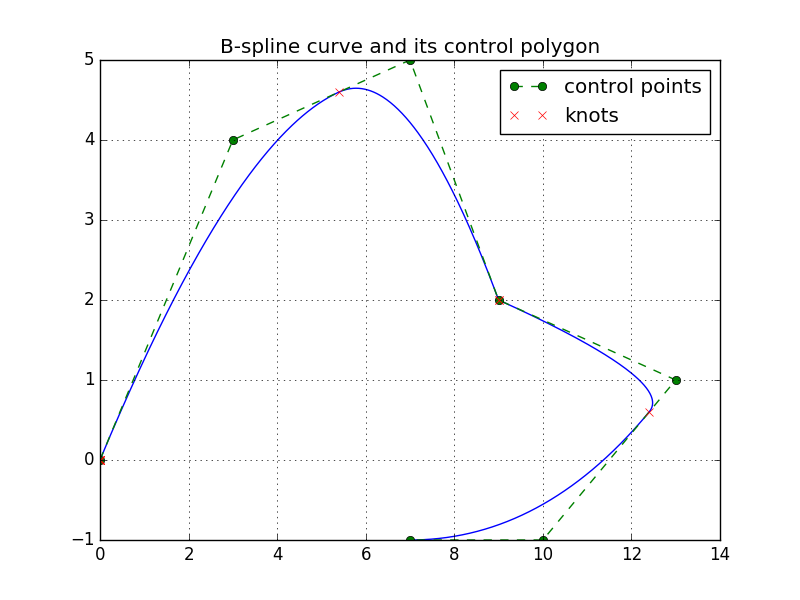
\includegraphics[scale=0.6]{bspline}
%\end{figure}

\section*{Task 3}
In this task we construct a circle using second degree NURBS and the de Boor algorithm. The code can be seen in Appendix I.\\
The following nine control points are used \begin{equation*}
\{(-1, 0), (-1, 1), (0, 1), (1, 1), (1, 0), (1, -1), (0, -1), (-1, -1), (-1, 0)\},
\end{equation*}
consisting of the vertices and midpoints of the unit square centered at $(0, 0)$ and its sides, respectively. As we want the curve to pass through the midpoints of the vertices and as these, apart from the starting point, will be situated at $\frac{1}{4}$, $\frac{2}{4}$ and $\frac{3}{4}$ of the whole curve, we need to include these points in the knot sequence with multiplicity two.\\
As we also want the curve to be clamped, this results in the knot sequence \begin{equation*}
\{0, 0, 0, 0.25, 0.25, 0.5, 0.5, 0.75, 0.75, 1, 1, 1\}.
\end{equation*}
If all weights are set to one, we end up with a B-spline curve with the following appearance

\begin{figure}[h!]
	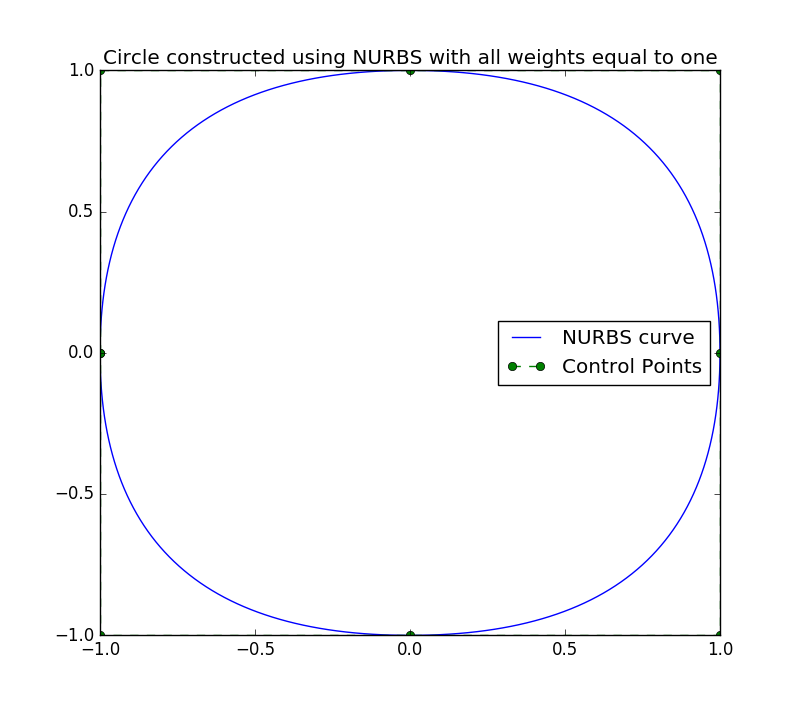
\includegraphics[scale=0.6]{splinecircle}
\end{figure}
In order to obtain an actual circle, we change the weights corresponding to the control points located in the vertices of the square. By trial and error, we find the correct weights $\omega$ to be \begin{equation*}
\omega= \{1, 0.707, 1, 0.707, 1, 0.707, 1, 0.707, 1\},
\end{equation*}
so the weights corresponding to the vertices of the square are approximately $\frac{\sqrt{2}}{2}$. The circle can be seen below.
\begin{figure}[h!]
	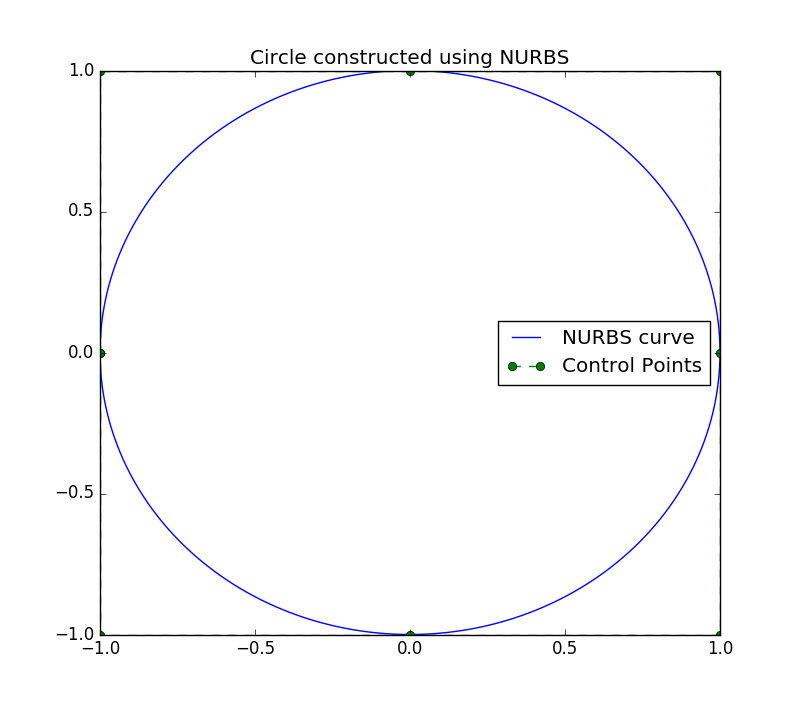
\includegraphics[scale=0.6]{nurbscircle}
\end{figure}
\section*{Do-over Homework 2 Task 5}
\underline{\textbf{Claim 1:}} The Lagrange form is invariant under all affine maps.\\
\\
\underline{\textbf{Proof:}} Let $\varphi:\mathbb{E}^n\rightarrow\mathbb{E}^n$ be any affine map. Then $\varphi$ can be expressed as \begin{equation*}
\varphi(u) = Au + v,
\end{equation*}
with $A\in\mathbb{R}^{n\times n}$ and $v\in\mathbb{R}^n$. Let $p$ be a polynomial of degree $n$. Then $p$ can be expressed as a linear combination of Lagrange basis polynomials $L_i^n$ of degree $n$, i.e. \begin{equation*}
p(x) = \sum_{i = 0}^{n}L_i^n(x)c_i,
\end{equation*}
with $c_i\in\mathbb{R}^n$ for $i = 0, 1, \dots, n$. Recall that the Lagrange basis fulfills the partition of unity, i.e. \begin{equation*}
\sum_{i = 0}^{n}L_i^n(x)=1.
\end{equation*}
We have that \begin{equation*}
\begin{aligned}
\varphi(p(x)) &= \varphi\left(\sum_{i = 0}^{n}L_i^n(x)c_i\right)\\
&= A\sum_{i = 0}^{n}L_i^n(x)c_i + v\\
&= \sum_{i = 0}^{n}L_i^n(x)Ac_i + v\\
&= \sum_{i = 0}^{n}L_i^n(x)Ac_i + 1\cdot v\\
&= \sum_{i = 0}^{n}L_i^n(x)Ac_i + \sum_{i = 0}^{n}L_i^n(x)v\\
&= \sum_{i = 0}^{n}L_i^n(x)(Ac_i + v)\\
&= \sum_{i = 0}^{n}L_i^n(x)\varphi(c_i)
\end{aligned}
\end{equation*}
which is what we wanted to show. $\square$\\
\\
\underline{\textbf{Corollary:}} The Lagrange form in invariant under all affine domain transformations.\\
\underline{\textbf{Proof:}} As all affine domain transformations are affine maps, the result follows directly from Claim 1. $\square$\\
\\
\underline{\textbf{Claim 2:}} The monomial form is \textbf{not} invariant under all affine domain transformations.\\
\\
\underline{\textbf{Proof:}} Let $\varphi:[c, d]\rightarrow [0, 1]$ be the affine domain transformation defined by \begin{equation*}
\varphi(u) = \frac{u - c}{d - c}
\end{equation*} 
and set \begin{equation*}
A=\frac{1}{d-c}, \quad v = \frac{c}{d - c},
\end{equation*}
so that \begin{equation*}
\varphi(u) = Au + v.
\end{equation*}
Now let $p$ be a polynomial of degree 1 on such that $\mathrm{Im}(p|_{[a, d]}) = [c, d]$. Then we can express $p$ as \begin{equation*}
\begin{aligned}
p(x) &= \sum_{i=0}^{1}x^ic_i\\
&=c_0 + xc_1, \quad x\in [a, b].
\end{aligned}
\end{equation*}
Then, for $x\in [a, b]$, \begin{equation*}
\begin{aligned}
\varphi(p(x)) &= \varphi(c_0 + xc_1)\\
&=A(c_0 + xc_1) + v
\end{aligned}
\end{equation*}
Furthermore, for $x\in [a, b]$, \begin{equation*}
\begin{aligned}
\sum_{i=0}^{1} x^i\varphi(c_i) &= \varphi(c_0) + x\varphi(c_1)\\
&=Ac_0 + v + x(Ac_1 + v)
\end{aligned}
\end{equation*}
Thus, for $x\in[a, b]$, $\varphi(p(x)) = \sum_{i = 0}^{1}x^i\varphi(c_i)$ iff $xv = 0$ which is not true in general. Hence, the monomial for is not invariant under all affine domain transformations. $\square$

\newpage
\section*{Appendix I}
\lstinputlisting{NURBSClass.py}

\end{document}
